\chapter{Introduction}
\label{ch:intro}

This document presents the smart store project which aims to make the shopping process easier and efficient for everyone. This document aims to give the related information needed to build the system with a planned and powerful way. The reader should be aware of the sections she/he needs refer to and investigate the document regarding the IEEE standards\cite{cite:ieee_2011_standards}, as well as having general knowledge on UML diagrams \cite{cite:booch_2004}\cite{cite:booch_2005}\cite{cite:siau_2007} and software design background. The standards in this book are mostly taken from the book of Sommerville \cite{cite:software_engineering_10}, any discrepancy should be cleared with the related section of the book.


\section{Purpose of the System}
The purpose of this project is to build the smart store project, namely "Amazon Go" \cite{cite:amazon_go_official}. "Amazon Go" project is a smart store project launched by Amazon whose objective is to present better, faster, and smarter shopping for everyone. In order to increase the automation along with the efficient use of resources, this project uses IoT and AI technologies to process data that come from sensors and cameras. This project diminishes the human error and inefficiency in the shopping process.

\section{Scope}

%Describe the scope of the software under consideration by
%a) Identifying the software product(s) to be produced by name (e.g., Host DBMS, Report Generator, etc.);
%b) Explaining what the software product(s) will do;
%c) Describing the application of the software being specified, including relevant benefits, objectives, and
%goals;
%d) Being consistent with similar statements in higher-level specifications (e.g., the system requirements
%specification), if they exist

This smart store project's aim is to provide a better, faster and safer environment for everyone in the shopping process as well as using resources efficiently. In order to
achieve such an environment for Amazon Go stores, the project shall have lots of
coordinated hardware and software components which are described below explicitly.

\begin{itemize}
    \item Since Amazon Go system needed to be maintained and improved, this system should have a technical staff. Objectives of this group will be explained in the related section.
    \item This technical staff group will have an interface to analyze system efficiently.
    \item System will have different kind of users. Thus, system will have store staff interface, customer interface and supplier interface as well. 
    \item Project will have lots of sensors/cameras that are scattered along store. In a very general view, these sensors provide the connection between customers and the system processing units.
    \item Project will have a great computational power since real time processing of incoming video stream is not an easy task.
    \item To process incoming data from both sensors and camera, project will have deep learning\&computer vision methods. Sensor fusion algorithms will be used as well.
    \item Project will have a database server running on the internal machines. These database table will be created with encryption methods.
    \item Lots of data needed to be transmitted in the system. Therefore, project will have connections between components. These connections should be trustworthy.
\end{itemize}

By this software, customers will use smart store like their refrigerators or their storage. They just come, take what they want and go out. There are no lines or any checkouts. It will be a huge benefit for customers. All of this huge work is done by automatizing the shopping process and making the store smarter.


\section{System Overview}

This section has information about the system overview. The factors affect and
components constitute the system are explained in depth.

\subsection{System Perspective}

Amazon Go is a smart store project which aims to reduce the human interference in purchasing process. This objective can't be reached without the help of computer and autonomous systems. Thus, Amazon Go uses computer vision algorithms, deep learning algorithms, and sensor fusion. Whole data captured by the sensors and cameras, which are spread throughout the market, is processed by the state of the art computer vision and deep learning algorithms.

There are outer components as well as the inner ones that interact with the Amazon Go system. Customers is one of the main actor that stimulates the system. As they purchase the products from the market, other parties involve or interact with the system also. For example, as long as the stocks are diminished under a predetermined threshold, the system sends new orders to the suppliers. These stock values are kept in a database system. Moreover, database system updated and checked automatically.

Although the system is designed as an autonomous system intentionally, there are human parts that contribute to the system execution as well. The technical staff is responsible for updating and maintaining the system, whereas the store staff is liable for supporting customers as well as cleaning \& organizing the market. Figure \ref{fig:context_diagram} shows this external entities as a context diagram.

\begin{figure} [H]
    \centering
    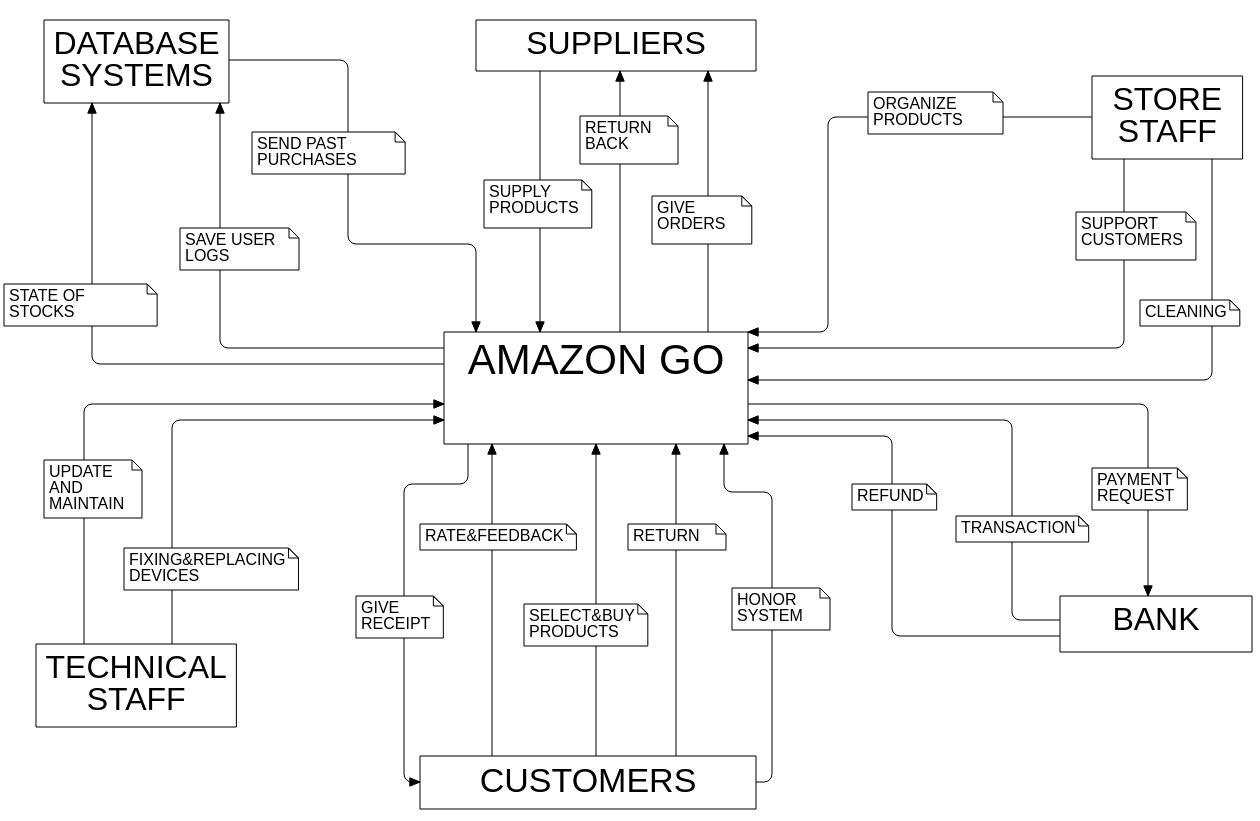
\includegraphics[width=\linewidth]{content/introduction/img/contextDiagram.png}
    \caption{Context Diagram}
    \label{fig:context_diagram}
\end{figure}

\subsection{System Functions}

 \begin{table}[H]
     \centering
     \begin{tabular}{ | l | p{10cm} |}
     \hline
     \textbf{Functionality}    & \textbf{Description} \\
     \hline
     Customer Support          & Store staff responds customer needs or requests. \\
     \hline
     Organize Products         & Store staff organizes the products in case of displacement of products. \\ 
     \hline
     Wrong Purchase Refund   &  A user requests a payback and get her/his refund from bank. \\
     \hline
     Payment                  & A customer pays his/her total debt. \\
     \hline
     Customer Preferences     & System analyzes customer preferences and uses that data for self progress. \\
     \hline
     Healthy Diet Analysis    & Users learn their dietary habit by analyzing his/her purchases. \\
     \hline
     Refund of Supply       & Store requests refund from the supplier.  \\
     \hline
     Supply  & Supplier supplies products to store and gets his/her payment from the store.\\
     \hline
     Credentials & Database function for keeping and retrieving customer credentials.\\
     \hline
     Analyze Logs & Technical staff views the system logs to maintain/develop system.\\
     \hline
     Device Replacement & Technical Staff replaces a non-operating electronic device. \\
     \hline
     Stock Control & Database system checks the stock condition of the products regularly.\\
     \hline
     \end{tabular} \caption{System Functions}
     \label{tab:01system_functions}
 \end{table}

\subsection{User Characteristics}
There are many users that are going to interact with the system. Therefore, the reader should consider different cases with different behaviours. The complete list of users of the system and their approximate profiles are :
\begin{itemize}
    \item Store staff
    \begin{itemize}
        \item Trained to use the system
        \item Not expected to be educated or technical
    \end{itemize}
    \item Technical staff
    \begin{itemize}
        \item Trained to use the system
        \item Having required technical knowledge on the system
        \item General system knowledge
    \end{itemize}
    \item Customers
    \begin{itemize}
        \item No education or training process present
        \item Some of which are lack of basic computer skills
        \item Basic understanding of shopping
        \item Any person in the world
    \end{itemize}
    \item Any person accompanying  the customer - same as the customers
    \item Data science analysts
    \begin{itemize}
        \item Enhanced knowledge on tools and database management
        \item Basic problem solving for software errors
        \item Experience with past and complicated systems
        \item Well educated and trained
    \end{itemize}
    \item Suppliers
    \begin{itemize}
        \item Trained to use the system
        \item No technical knowledge
        \item Very limited computer skills
    \end{itemize}
\end{itemize}

\subsection{Limitations}
% regulatory policies -> sanki personal information gibi degil
\begin{itemize}
    \item \textbf{Regulatory policies:} In the system, personal information exists such as name, surname, address and phone number. What's worse is that credit card information of customers are involved in the system although the system kept these private information in an encrypted way with the state of the art security techniques. Thus, any of the system data should not be released to public access. 
    \item\textbf{Hardware limitations:} Firstly, there is no hardware dependency or hardware usage for customers except a smartphone. An Android or Ios powered smartphone which can run the system's customer app is sufficient. For the system side, a high computation power is needed since the system does real time image processing with computer vision\&deep learning algorithms. Also, system should consider and evaluate incoming data from hundreds of sensors. The system is also dependent to these sensor devices. Naturally, these whole devices should be connected to each other with a secure local area network. Some of the parts of the system should also connected to the outside as well. Therefore, system itself is highly dependent to the hardware and if one component of the system does not work as expected, system might be crashed.       
    \item\textbf{Interfaces to other applications:} Since Amazon Go smart store project has all
    necessary systems to operate, it doesn't have an interface to other applications. 
    \item\textbf{Parallel operations:} All cameras and sensors need to operate all the time while the store is open to customers. Since these whole incoming data should be processed at every
    moment , the system should be capable to serve all processing units at the same time. That means, parallelization is a must in this system.
    \item\textbf{Audit functions:} Accounts of store staff and technical staff are controlled by Amazon Go smart store system, therefore there is a need for audit functions .
    \item\textbf{Control functions:} Database can only accessible for authorized staff. Non-authorized people cannot change/retrieve any data in the database. Also, interfaces for customer, technical staff, store staff and supplier should be secure. 
    \item\textbf{High-order language requirements:} Project should use web based systems so appropriate languages such as JavaScript and HTML can be used.In the database side , SQL should be used. Also, for other purposes, languages that are not machine dependent such as Java can be used since lots of hardware devices exist in project.
    \item\textbf{Signal handshake protocols:} Since the system uses web, HTTPS will be required.Also TCP/IP services can be used when there is a connection created between two devices.
    \item\textbf{Quality requirements:} Safety and reliability of the system are really crucial.For that purposes, staff should take backups of logs and should control security of system regularly.
    \item\textbf{Criticality of the application:} Since the system is not used for medical or security purposes and there is no danger for anyone's health if the system is crashed, the system might be categorized as not critical. However, system crashes might result in a big economic losses. From this point of view, system should work as intended and it can be said that it is critical.
    \item\textbf{Safety and security considerations:} Technical staff should keep
    system protected from malicious users/unauthorized people.
    \item\textbf{Physical/mental considerations:} Any person who are able to shop
    from other markets, can shop from Amazon Go smart store, even in an easy way. Store should also be organized in such a way that walking disabled people can reach all products. 
\end{itemize}



\section{Definitions}

\begin{table}[H]
    \centering
    \begin{tabular}{ | l | p{10cm} |}
    \hline
    \textbf{Technical Staff}    & Person whose job is related to “information technology”. \\
    \hline
    \textbf{Database}           & Organized collection of data. \\
    \hline
    \textbf{HTTPS}      & “Hyper Text Transfer Protocol Secure is a protocol for secure communication over network which is widely used on web.\\
    \hline
    \textbf{HTML}             & “Hypertext Markup Language” is the standard markup language for creating web pages and web applications. \\
    \hline
    \textbf{SQL}    & "Structured Query Language" is a domain-specific language used in programming and designed for managing data held in a relational database management system. \\
    \hline
    \textbf{IoT}         & Internet of Things, a system of interrelated computing devices which have capability to transfer measured data over a network. \\
    \hline
    \textbf{TCP/IP}         & One of the main protocols of the Internet protocol suite which provides reliable, ordered, and error-checked delivery \\
    \hline
    \end{tabular}
    \label{tab:defitinions}
    \caption{Definitions Table}
\end{table}